\documentclass{article}

\usepackage{arxiv}

\usepackage[utf8]{inputenc} % allow utf-8 input
\usepackage[T1]{fontenc}    % use 8-bit T1 fonts
\usepackage{lmodern}        % https://github.com/rstudio/rticles/issues/343
\usepackage{hyperref}       % hyperlinks
\usepackage{url}            % simple URL typesetting
\usepackage{booktabs}       % professional-quality tables
\usepackage{amsfonts}       % blackboard math symbols
\usepackage{nicefrac}       % compact symbols for 1/2, etc.
\usepackage{microtype}      % microtypography
\usepackage{graphicx}

\title{Current state and prospects of R-packages for the design of
experiments}

\author{
    Emi Tanaka
    \thanks{Corresponding author}
   \\
    Department of Econometrics and Business Statistics \\
    Monash University \\
  Clayton, VIC 3800 \\
  \texttt{\href{mailto:emi.tanaka@monash.edu}{\nolinkurl{emi.tanaka@monash.edu}}} \\
   \And
    Dewi Amaliah
   \\
    Department of Econometrics and Business Statistics \\
    Monash University \\
  Clayton, VIC 3800 \\
  \texttt{} \\
  }


% tightlist command for lists without linebreak
\providecommand{\tightlist}{%
  \setlength{\itemsep}{0pt}\setlength{\parskip}{0pt}}


% Pandoc citation processing
\newlength{\cslhangindent}
\setlength{\cslhangindent}{1.5em}
\newlength{\csllabelwidth}
\setlength{\csllabelwidth}{3em}
\newlength{\cslentryspacingunit} % times entry-spacing
\setlength{\cslentryspacingunit}{\parskip}
% for Pandoc 2.8 to 2.10.1
\newenvironment{cslreferences}%
  {}%
  {\par}
% For Pandoc 2.11+
\newenvironment{CSLReferences}[2] % #1 hanging-ident, #2 entry spacing
 {% don't indent paragraphs
  \setlength{\parindent}{0pt}
  % turn on hanging indent if param 1 is 1
  \ifodd #1
  \let\oldpar\par
  \def\par{\hangindent=\cslhangindent\oldpar}
  \fi
  % set entry spacing
  \setlength{\parskip}{#2\cslentryspacingunit}
 }%
 {}
\usepackage{calc}
\newcommand{\CSLBlock}[1]{#1\hfill\break}
\newcommand{\CSLLeftMargin}[1]{\parbox[t]{\csllabelwidth}{#1}}
\newcommand{\CSLRightInline}[1]{\parbox[t]{\linewidth - \csllabelwidth}{#1}\break}
\newcommand{\CSLIndent}[1]{\hspace{\cslhangindent}#1}

\usepackage{colortbl}
\usepackage{bera}
\usepackage{xcolor}
\usepackage{hyperref}
\usepackage[utf8]{inputenc}
\def\tightlist{}
\newcommand{\ctv}[1]{\href{http://CRAN.R-project.org/view=#1}{\emph{#1}}}

\begin{document}
\maketitle


\begin{abstract}
Re-running an experiment is generally costly and in some cases
impossible due to limited resources, so the design of an experiment
plays a critical role in increasing the quality of experimental data. In
this paper we describe the current state of the R-packages for the
design of experiments through an exploratory data analysis of package
downloads, package metadata, and the comparison of characteristics with
other topics. We observe that experimental designs in practice appear to
be sufficiently manufactured by a small number of packages and the
development of experimental designs often occur in silos. We discuss
also the interface designs of widely utilised R packages in the field of
experimental design and discuss its future prospects to advance the
field in practice.
\end{abstract}


\hypertarget{introduction}{%
\section{Introduction}\label{introduction}}

The critical role of data collection is well captured in the expression
``garbage in, garbage out'' -- in other words, if the collected data is
rubbish then no analysis, however complex it may be, can make something
out of it. A carefully crafted data collection scheme is therefore
critical to optimise the information from data. The field of
experimental designs is specifically devoted to planning the collection
of experimental data, largely based on the founding principles by Fisher
(1935) or an optimisation framework like those described in Pukelsheim
(2006). These experimental designs are often constructed with the aid of
a statistical software, such as R (R Core Team 2021), Python (Rossum
1995), SAS (SAS Institute 1985), and so on, so the usage of experimental
design software can inform us about some aspects of experimental designs
in practice.

Methods for data collection can be dichotomised by the type of data
collected -- namely, experimental or observational -- or alternatively,
categorised as experimental design (including quasi-experimental design)
or survey design. This dichotomisation, to a great extent, is seen in
the \href{https://cran.r-project.org/web/views/}{Comprehensive R Archive
Network (CRAN) task views} (a volunteer maintained list of R-packages by
topic) where R-packages for experimental design are in
\href{http://CRAN.R-project.org/view=ExperimentalDesign}{\emph{ExperimentalDesign}}
task view and R-packages for survey designs are in
\href{http://CRAN.R-project.org/view=OfficialStatistics}{\emph{OfficialStatistics}}
task view. The full list of available topics can be see in Table S1 in
the Supplementary Materials. A subset of experimental designs are
segregated into
\href{http://CRAN.R-project.org/view=ClinicalTrials}{\emph{ClinicalTrials}}
task view, where the focus is on clinical trials with primary interest
in sample size calculations. This paper focuses on the packages in
\href{http://CRAN.R-project.org/view=ExperimentalDesign}{\emph{ExperimentalDesign}}
task view, henceforth referred to as ``DoE packages''.

In
\href{http://CRAN.R-project.org/view=ExperimentalDesign}{\emph{ExperimentalDesign}}
task view, there are 114 R packages for experimental design and analysis
of data from experiments. The sheer quantity and variation of
experimental designs in the R-packages are arguably unmatched with any
other programming languages, e.g.~in Python, only a handful of packages
that generate design of experiment exist (namely \texttt{pyDOE},
\texttt{pyDOE2}, \texttt{dexpy}, \texttt{experimenter} and
\texttt{GPdoemd}) with limited type of designs. Thus, the study of DoE
packages, based on quantitative and qualitative data, can give us an
objective view to the state of the current experimental designs in
practice.

A utility of software can also be described by its design to facilitate
clear expression and interpretation of the desired experimental design.
Certain programming language design can hinder or discourage development
of a reliable program (Wasserman 1975). The immense popularity of
\texttt{tidyverse} (a collection of R-packages for various stages of
data analysis that place enormous emphasis on the interface design by
Wickham et al. 2019) is a testament to the impact an interface design
can have in practice. The practice of experimental design could be
advanced by adopting similar interface design principles across DoE
packages.

The paper is organised as follows. Section \ref{data} briefly describes
the data source used for the analysis in Section \ref{eda}; Section
\ref{eda} presents some insights into the state of the current DoE
packages by the exploratory data analysis of package download data, text
descriptions and comparisons with other CRAN task views; Section
\ref{design} discusses the interface designs of widely used DoE
packages, and we conclude with a discussion in Section \ref{discussion}
of future prospects in the software development of experimental designs.

\hypertarget{data}{%
\section{Data}\label{data}}

To study the DoE packages, we analyse data using three sources of data
as described below.

\hypertarget{rstudio-cran-download-logs}{%
\subsection{RStudio CRAN download
logs}\label{rstudio-cran-download-logs}}

The Comprehensive R Archive Network (CRAN) is a network of servers
located across the world that store mirrored versions of R and
R-packages. The most popular network is the RStudio mirror (the default
server for those that use the RStudio IDE). The RStudio mirror is also
the only server that provides a comprehensive daily download logs of R
and R-packages since October 2012. The summary data can be easily
accessed with the \texttt{cranlogs} package (Csárdi 2019). This paper
uses the data from the beginning of 2013 to end of 2021 (a total of 9
years) for the packages in the CRAN task views.

\hypertarget{package-descriptions}{%
\subsection{Package descriptions}\label{package-descriptions}}

All CRAN packages have a title, description, package connections
(suggests, depends and imports) and other meta-information in the
DESCRIPTION file. We use the text data from the title and description
(as accessed in 2022-05-23) in Section \ref{topics}.

\hypertarget{cran-task-views}{%
\subsection{CRAN task views}\label{cran-task-views}}

CRAN task views are volunteer maintained list of R-packages on CRAN
relevant to the corresponding topic. There are a total 37 CRAN task
views. Table S1 in the Supplementary Materials list the full available
topics from the \texttt{ctv} package (Zeileis 2005). The list of
packages in each CRAN task views (as of 2022-05-25) are used to contrast
the characteristics of DoE packages in Sections \ref{popular} and
\ref{silo}.

\hypertarget{eda}{%
\section{Explorative data analysis}\label{eda}}

In this section, we derive some conjecture based on the analysis of the
data described in Section \ref{data}. All results presented are from the
exploratory data analysis of observational data, consequently, all
interpretations are somewhat speculative and may not be indicative of
the true state of the field of experimental design. In particular, any
analysis over time are confounded by the fact that the nature of users
and package management have also changed over the years. It should be
noted that some DoE packages may have been archived or removed from the
task view over the years so any cross-sectional analysis presented may
not reflect the set of all DoE packages at that particular time period
(although we assume such incidences are low).

A subset of DoE packages is not primarily about design of experiments
but about the analysis of experimental data. A complete delineation of
these packages is difficult as there is almost always at least one
function that can aid decisions or constructions of experimental designs
(and any categorisation is prone to our subjective bias) so we opted not
to remove any DoE packages in the analysis.

\hypertarget{popular}{%
\subsection{Small, but diverse, set of packages are sufficient for most
experimental designs in practice}\label{popular}}

There have been at least 50 DoE packages since 2013 but most of the
downloads are concentrated in just a handful of packages. For example,
Figure \ref{fig:plot-lorenz} shows a Lorenz curve (Lorenz 1905) for the
total package downloads in 2021 of 113 DoE packages (first released
prior to 2021); we can see from Figure \ref{fig:plot-lorenz} that bottom
90\% of DoE packages (in terms of total download count in 2021) only
share about 30\% of total downloads across all DoE packages -- in
another words, 70\% of the total downloads are due to 11 packages (10\%
of the DoE packages).

\begin{figure}[htbp]

{\centering 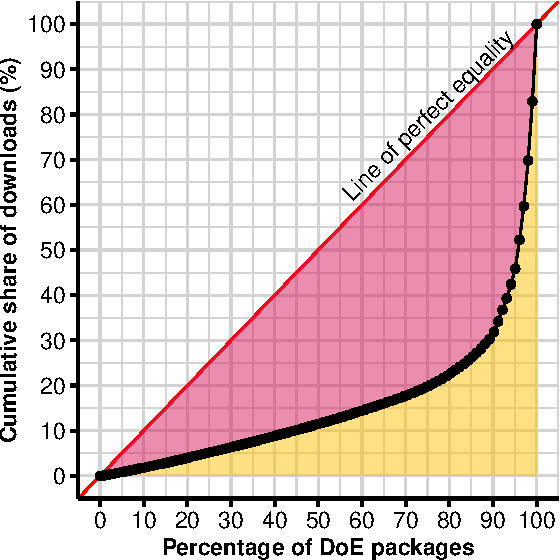
\includegraphics{figures/plot-lorenz-1} 

}

\caption{Lorenz curve of the total download count for DoE packages in 2021. The red line corresponds to the line of perfect equality. The green region shows the area under the Lorenz curve and the red region shows the area of gap in equality.}\label{fig:plot-lorenz}
\end{figure}

If we consider package downloads as a measure of ``wealth'', then we can
consider using the Gini index (Gini 1921) as a measure of download
inequality across packages. The ratio of the red region over the total
colored regions in Figure \ref{fig:plot-lorenz} corresponds to the Gini
index for 2021. A Gini index of 0\% indicates equality in downloads
across packages while a value of 100\% indicates maximal inequality (all
downloads are due to one package). In Figure \ref{fig:download-share},
we see that the distributions of the package downloads each year have a
heavy right tail with the Gini index ranging from 42.6\% to 74.1\%
across the years 2013 to 2021, indicating that there is a high level of
inequality of package downloads, particularly with more pronounced
inequality in the last 6 years.

\begin{figure}[htbp]

{\centering 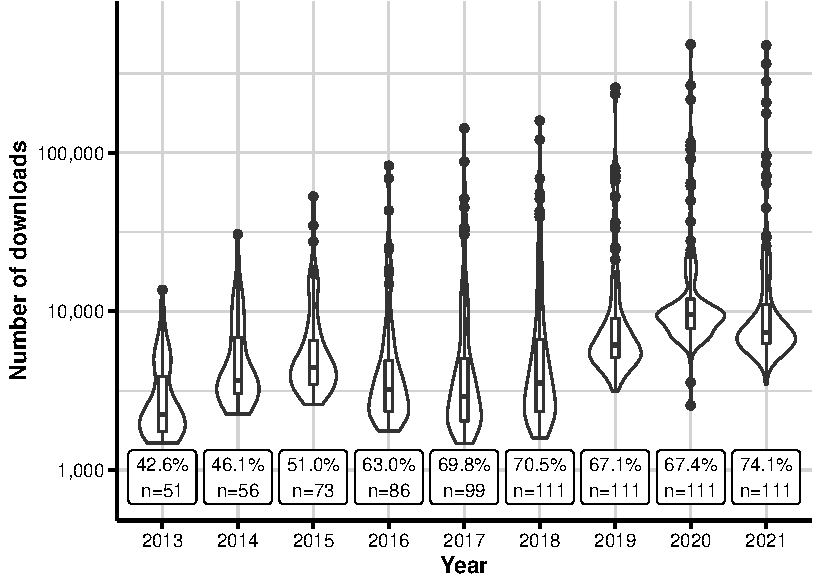
\includegraphics{figures/download-share-1} 

}

\caption{The distribution of the number of downloads for each DoE package by year. Packages were removed in any year if it was released in that year or later so that each download count is for the full year. The label on the bottom of the plot shows the Gini index for downloads and the number of packages with full year of download count in the corresponding year. In the last 6 years, the Gini index is consistent above 60\% each year indicating that most downloads are due to a relatively small number of packages. }\label{fig:download-share}
\end{figure}

The increase in the number of packages that are not highly downloaded
may mean that \textbf{\emph{there are more packages to construct niche
experimental designs}}. Some examples of these packages include
\texttt{qtlDesign}, \texttt{PwrGSD} and \texttt{Crossover} made for QTL
experiments, group sequential designs and crossover trials,
respectively. These packages would naturally have a smaller number of
potential users. Counterfactual to this, the increase could be due to
other external factors, such as an increase in the number of skilled
developers (and thus more pacakge contributions), a change in CRAN
policy or management to add packages (either to CRAN and/or task view),
and/or that new packages are still yet to amass users. While there is an
argument that low download counts are due to the low utility and/or
quality of the packages, packages in CRAN task views are selected by
expert maintainers, thus we can reasonably assume that any package
listed in CRAN task view are of a decent utility and quality.

If the downloads are reflective of the experimental designs used in
practice, \textbf{\emph{small set of packages appear to be sufficient
for most to construct the full set of designs of experiments needed in
practice}}. Packages of course evolve and the top downloaded packages
have had regular updates that may have broadened its scope from its
previous releases.

While in absolute terms the Gini index is high for
\href{http://CRAN.R-project.org/view=ExperimentalDesign}{\emph{ExperimentalDesign}}
task view (42.6\% to 74.1\%), the inequality is not as severe as other
CRAN task views as shown in Figure \ref{fig:fig-gini-all-ctvs}. We can
see in Figure \ref{fig:fig-gini-all-ctvs} that the Gini index is
generally increasing for DoE packages (as is generally the case for
other CRAN task views as shown in Figure S1 in the Supplementary
Materials) but most other CRAN task views have a Gini index of over
75\%. This suggests that other CRAN task views may have dominant
standards and in comparison to other topics, there are more
\textbf{\emph{diverse approaches to designing experiments}} and thus no
single DoE package is dominant. This observation however doesn't take
into account other approaches to generating experimental designs, like
the proprietary software, CycDesignN (Whittaker, Williams, and John
2022) and SAS (SAS Institute 1985), which may be widely used.

\begin{figure}[htbp]

{\centering 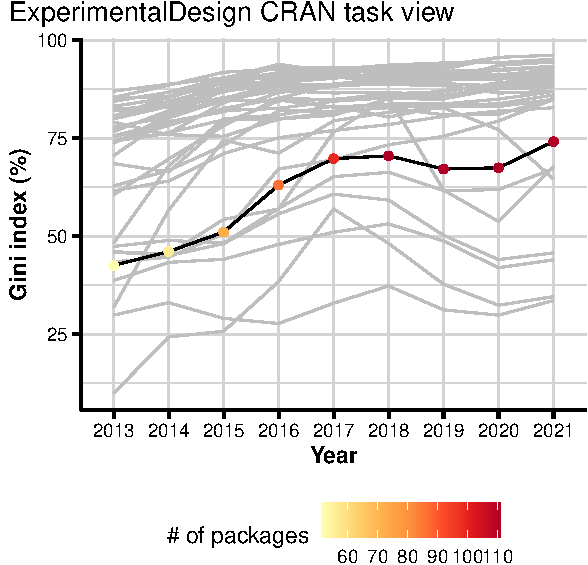
\includegraphics{figures/fig-gini-all-ctvs-1} 

}

\caption{The points show the Gini index of the download counts by year for ExperimentalDesign task view with the color showing the number of packages. The grey line shows the distribution of the Gini index across years for all other CRAN task views. See Figure S1 in the Supplementary Material for the line graph for the Gini index across years by each CRAN task view.}\label{fig:fig-gini-all-ctvs}
\end{figure}

\hypertarget{ranking}{%
\subsection{The field of experimental design is
slow-changing}\label{ranking}}

We can see in Figure \ref{fig:rank-over-time} that most of the top 10
ranking packages have been in the top 10 for the last 9 years with
\texttt{lhs} steadily climbing up the ranks in the last few years. It
should be noted that the download of one package can prompt a download
of another package; the most notable dependency network is
\texttt{AlgDesign} and \texttt{agricolae}, where the former is an import
for the latter. The full dependency network within the DoE packages is
shown later in Figure @ref(fig:plot-doe-network).

\begin{figure}[htbp]

{\centering 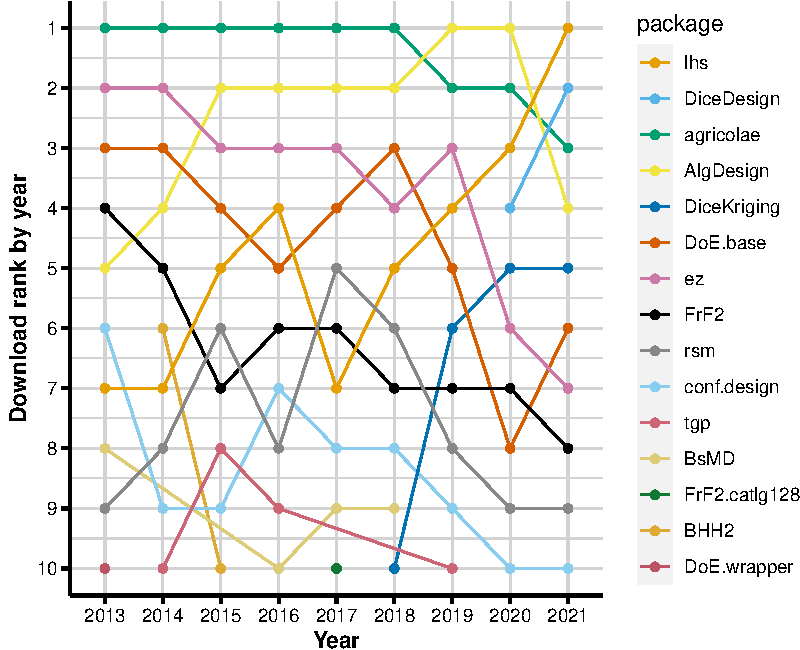
\includegraphics{figures/rank-over-time-1} 

}

\caption{The plot shows the rank of top 10 downloaded packages by year. Packages that do not appear in top 10 for at least two periods are omitted from the plot. Most packages are consistently in the top 10 for the period shown.}\label{fig:rank-over-time}
\end{figure}

Figure \ref{fig:release-date-vs-download} shows a moderate negative
correlation between the first release date and the (log of) total
download counts of DoE packages in any given year from 2013 to 2021.
This suggest that in general, a package released earlier are more likely
to be used today (possibly for legacy reasons or the general inertia to
adopt new packages). We can also see in Figure
\ref{fig:release-date-vs-download} the most downloaded packages were
generally released in 2004 to 2010.

\begin{figure}[htbp]

{\centering 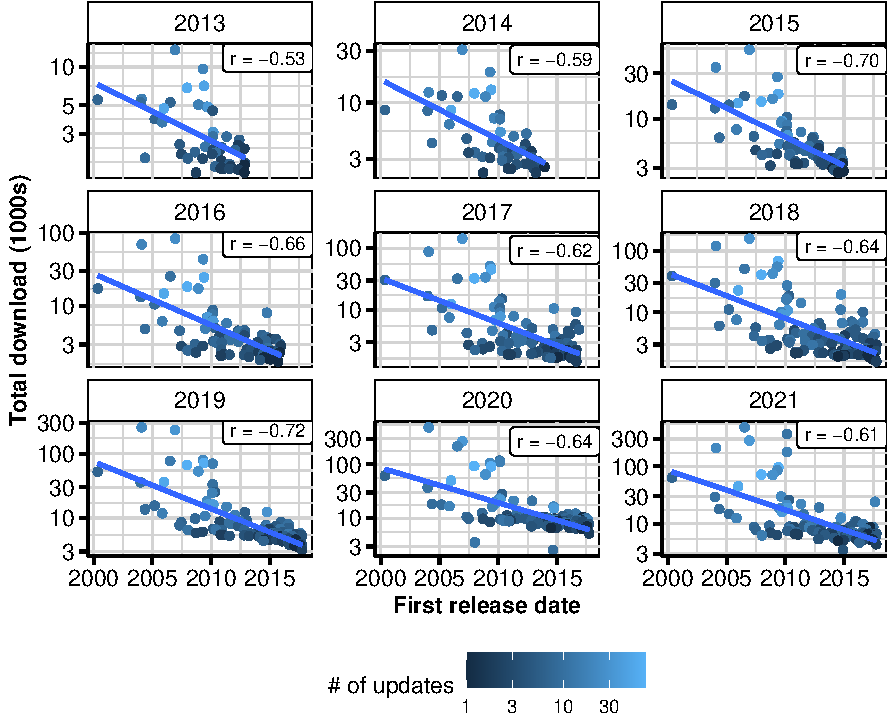
\includegraphics{figures/release-date-vs-download-1} 

}

\caption{The above figure shows the total download (in log scale) of a package in the corresponding year against the first release date of the package. The blue line corresponds to the least squares fit of a simple linear regression model. The label in the right-hand upper corner shows the sample correlation coefficient between the first release date and the log (with base 10) of the total download count. The high-leverage point on the far left belongs to `conf.design`, authored by one of the earlier contributors to R.}\label{fig:release-date-vs-download}
\end{figure}

The consistency in the top 10 ranking packages (Figure
\ref{fig:rank-over-time}) and the fact that most downloaded DoE packages
are first released more than 10 years ago (Figure
\ref{fig:release-date-vs-download}) indicates that either the existing
packages filled the needs of mass in practice or no new packages were
compelling for many to switch their practice. We do however also see
that the the top downloaded packages generally have more updates (see
Figure \ref{fig:release-date-vs-download}) so it is possible that the
packages have improved or broadened the scope of its usage.

\hypertarget{topics}{%
\subsection{Optimal designs are of interest}\label{topics}}

Figure \ref{fig:wordcloud-over-time} shows some common purposes of DoE
packages, based on bigrams in the package title and description. We show
only the bigrams as unigram was not insightful and there were not many
trigrams common across packages. In counting the bigrams, we processed
the text data as follows:

\begin{enumerate}
\def\labelenumi{\arabic{enumi}.}
\tightlist
\item
  We standardised the words to lower case and removed pluralization.
\item
  Multiple mentions of the same bigram within a package was counted as
  one (e.g.~\texttt{AlgDesign} mentions ``experimental design'' four
  times in the title and the description but this is counted as one).
\item
  Bigrams that consist the stop words (provided in
  \texttt{tidytext::stop\_words} in addition to other words we deemed
  irrelevant, e.g.~``provide'', ``e.g.'', ``calculate'' and so on; full
  list is shown in the code provided in the link under Section
  \ref{pkgs}) are removed.
\end{enumerate}

Not surprisingly, the bigram ``experimental design'' was the most
common. More interestingly, ``optimal design'' and ``sequential design''
appeared across different packages (indicated by the size of the word in
Figure \ref{fig:wordcloud-over-time}), and the bigrams ``latin
hypercube'' and ``computer experiment'' are used across a few packages
that are downloaded frequently (indicated by the color of the word in
Figure \ref{fig:wordcloud-over-time}). Sequential design, Latin
hypercube sampling and computer experiments (which generally include
space filling designs like Latin hypercube sampling) are designs that
generally operate by optimising a user-selected criterion and can be
classified as optimal designs.

\begin{figure}[htbp]

{\centering 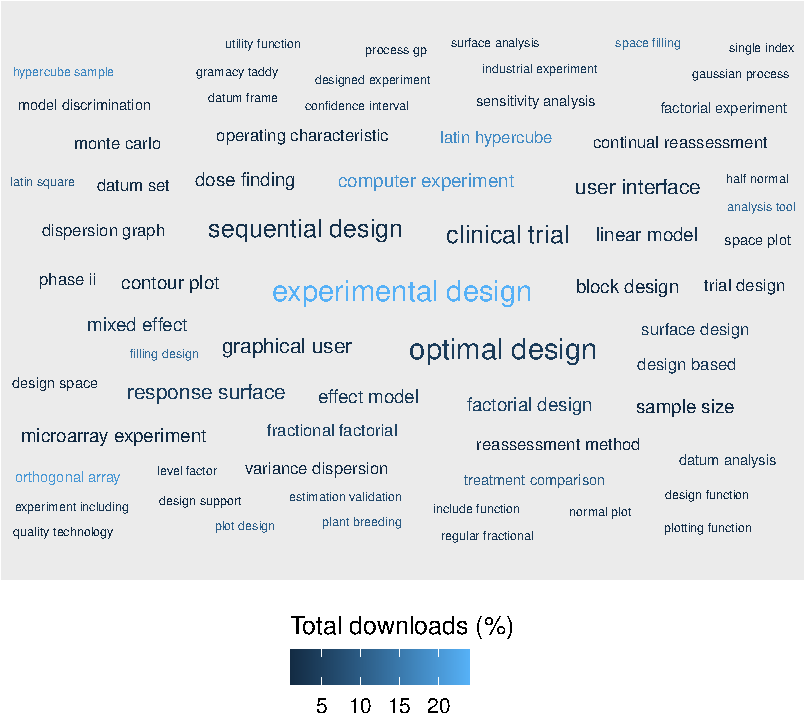
\includegraphics{figures/wordcloud-over-time-1} 

}

\caption{The above figure shows the word cloud of bigrams from the title and descriptions of the DoE packages. The size shows how often the bigram appears across the DoE packages and the color are relative to the total download count in 2021 of the packages that contain the bigram.}\label{fig:wordcloud-over-time}
\end{figure}

Although there exists a separate
\href{http://CRAN.R-project.org/view=ClinicalTrials}{\emph{ClinicalTrials}}
task view, the DoE packages clearly include some packages that are of
interest to clinical trials as shown by the size of the bigram
``clinical trial'' (and related bigrams like ``dose finding'' and
``phase ii'') in Figure \ref{fig:wordcloud-over-time}.

\hypertarget{silo}{%
\subsection{Development of experimental designs occur in
silos}\label{silo}}

Figure \ref{fig:ctv-summ-plot} shows that the
\href{http://CRAN.R-project.org/view=ExperimentalDesign}{\emph{ExperimentalDesign}}
task view has the lowest average number of contributors among all 37
CRAN task views. In addition, we can also see in Figure
\ref{fig:ctv-summ-plot} that the
\href{http://CRAN.R-project.org/view=ExperimentalDesign}{\emph{ExperimentalDesign}}
task view has one of the least intra-connectivity (the percentage of
packages that make use of other packages within the same task view). The
full connection of DoE packages with other DoE packages is shown in
Figure \ref{fig:plot-doe-network}. These observations suggest that the
\textbf{\emph{field of experimental design is one of the least
collaborative field}} and package development generally occur in silos.

\begin{figure}[htbp]

{\centering 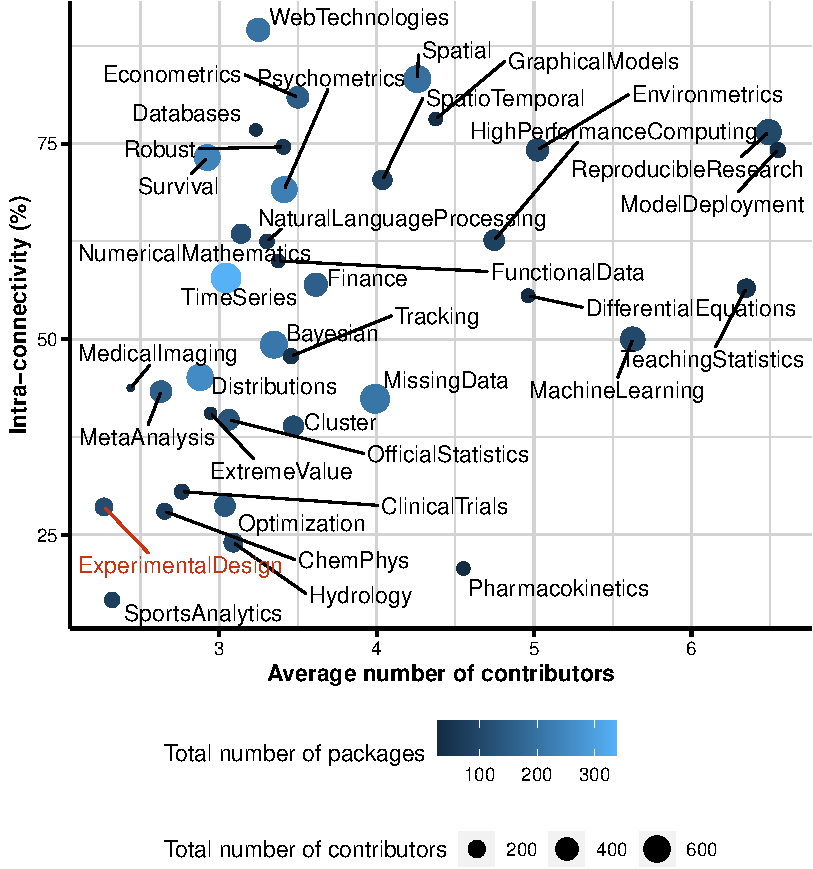
\includegraphics{figures/ctv-summ-plot-1} 

}

\caption{The above figure is a scatterplot of the intra-connectivity (the percentage of packages that depends, suggest or imports at least one other package within the same task view) and the average number of contributors for each CRAN task view. A low intra-connectivity suggests that development within the topic mostly occur in silos whilst high  intra-connectivity suggests that there are more interactions within the topic. The color shows the number of packages, the size of the point corresponds to the total number of contributors, and the text labels show the CRAN task view name.  The label of ExperimentalDesign task view is colored red. The task views in the bottom-left corner are topics that are more indicative of contributors working in silos. The actual numerical values are show in Table S1 in the Supplementary Material.}\label{fig:ctv-summ-plot}
\end{figure}

\begin{figure}[htbp]

{\centering 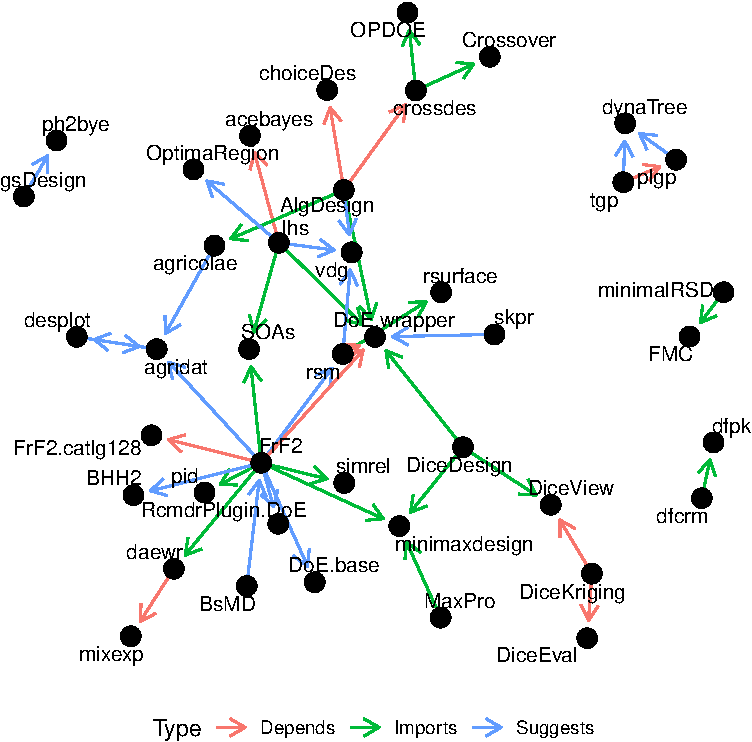
\includegraphics{figures/plot-doe-network-1} 

}

\caption{Package connections (depends, suggests and imports) within the DoE packages. The direction of the arrow shows the connection of packags where the package on the tail of the arrow is a depedency, suggestion or import for the package on the head of the arrow.  DoE packages that do not depend, suggest or import another DoE package is not shown.}\label{fig:plot-doe-network}
\end{figure}

\hypertarget{design}{%
\section{Interface design}\label{design}}

In software design, there are two interface designs to consider: user
interface (UI) and application programming interface (API). UI is
concerned with the interaction of the software by the user, while the
API is concerned with how different programs interact and is
predominately of the interest to the developer. The UI design is an
abstraction to specifying the desired experimental design and its
choices enable how a user expresses the specification of the
experimental design. The API design aids in other developers to leverage
existing systems.

In this section, we discuss these interface designs broadly, with
examples illustrated from the top downloaded packages (shown in Figure
\ref{fig:rank-over-time}). We exclude \texttt{ez} and
\texttt{DiceKriging} from the discussion as the former is predominately
visualisation of experimental data and the latter is about the analysis
of computer experiments in addition to belonging to the same suite of
packages as \texttt{DiceDesign} (Dupuy, Helbert, and Franco 2015).

\hypertarget{the-case-of-factorial-designs}{%
\subsection{The case of factorial
designs}\label{the-case-of-factorial-designs}}

Factorial experiments offer a challenge in the construction and
allocation of the treatment factors. This is reflected in a number of
packages that specifically addresses this challenge. These include
\texttt{DoE.base} (Grömping 2018) for full factorial and (regular and
irregular) orthogonal array designs via \texttt{fac.design()} and
\texttt{oa.design()}, respectively, \texttt{FrF2} (Grömping 2014) for
fractional 2-level factorial designs using \texttt{FrF2()},
\texttt{FrF2Large()} or \texttt{pb()} Plankett-Burnman designs (Plackett
and Burman 1946), \texttt{conf.design} (Venables 2013) for symmetric
confounded factorial designs via \texttt{conf.design()}, and
\texttt{BHH2} (Barrios 2016) to generate full or fractional 2-level
factorial design matrix via \texttt{ffDesMatrix()}. All these designs
generally requires the user to input the number of factors and if the
design is allowed to vary in the number of levels, the input of the
number of levels for each factor. The construction of some of these
designs are catalogue-based, e.g.~\texttt{oa.design()} in
\texttt{DoE.base}.

Response surface design, as illustrated by \texttt{rsm} (Lenth 2009), is
a factorial experiment but the focus of it is to analyse using response
surface modelling. The two well known response surface designs are
Box-Behnken design (Box and Behnken 1960) and central-composite designs
(Box and Wilson 1951) via \texttt{bbd()} and \texttt{ccd()} for
central-composite designs providing formula.

Saturated designs

\hypertarget{the-case-of-menu-designs}{%
\subsection{The case of menu designs}\label{the-case-of-menu-designs}}

Computer experiments, as discussed in Section \ref{topics}, which
generally involve space filling designs, have been on the rise. The
exemplar for this type of designs are \texttt{lhs} (Carnell 2022) and
\texttt{DiceDesign}. For the \texttt{lhs} package, functions like
\texttt{randomLHS()}, \texttt{optimumLHS()}, and \texttt{maximinLHS()},
require users to specify the sample size (\(n\)) and the number of
variables (\(p\)) then it generates a Latin hypercube sample, based on
different optimisation schemes (in this case, random, S optimal and
maxmin criteria, respectively; see package documentation for more
details). Similarly for the \texttt{DiceDesign}, there is a
comprehensive list of space-filling designs such as
\texttt{dmaxDesign()}, \texttt{lhsDesign()}, \texttt{straussDesign()}
and \texttt{wspDesign()} with input of \(n\) and \(p\) as before (among
extra parameters for some) that implement algorithms that either
maximise the entropy, produce a random Latin hypercube sample, based on
Strauss process and WSP algorithm, respectively. These designs all
output a \(n \times p\) matrix with values between 0 and 1.

The \texttt{AlgDesign} (Wheeler 2022) package offers three primary
functions for generating optimal designs: \texttt{optBlock()},
\texttt{optFederov()} and \texttt{optMonteCarlo()}. These functions in
general require a formula in terms of the supplied terms with the choice
of criterion (D, A and I for the latter two). The difference lies in the
search algorithm for the optimal design.

The \texttt{agricolae} package (de Mendiburu 2021) was the most
downloaded DoE packages in 2013 to 2018 (Figure
\ref{fig:rank-over-time}) and possibly prior to 2013 (data unavailable).
This package is the prime example of constructing designs based on menu
functions, e.g.~\texttt{design.crd()}, \texttt{design.rcbd()} and
\texttt{design.split()} construct a completely randomised design,
randomised complete block design and split-plot design, respectively.
Users typically supply the treatment labels (or number of treatments in
the case of \texttt{design.split()}) and the number of replications as
argument to these functions.

\hypertarget{the-case-of-sequential-designs}{%
\subsection{The case of sequential
designs}\label{the-case-of-sequential-designs}}

Another specialised design is sequential design (also called adaptive
sampling), which is best represented by \texttt{tgp} (Gramacy and Taddy
2010) -- these require prior information, which are used to inform the
next experimental design using \texttt{tgp.design()} and
\texttt{dopt.gp()} which requires users to supply candidate samples to
sub-sample from and a model or design from a prior design. Follow-up
experiments, which can also be classified as a sequential design, is
implemented by \texttt{BsMD} (Barrios 2020). In \texttt{BsMD}, the
follow-up design is determined by a model discriminant approach using
\texttt{MD()}.

\hypertarget{discussion}{%
\section{Discussion}\label{discussion}}

Through the exploratory data analysis of three data sources (package
download logs, package metadata and CRAN task views) outlined in Section
\ref{data}, we have observed that the the total download of DoE packages
are concentrated only on a handful of R-packages although these
represent a diverse set in comparison with other CRAN task views.
Furthermore, the data suggests that the field of experimental design is
the least collaborative field; out of all CRAN task views, it has one of
the least average number of authors and the lowest intra-connectivity
(any dependency on other packages within its own task view). There are a
number of limitations and short coming in our exploratory data analysis.
First, CRAN task views are volunteer maintained so some experimental
design packages may not be included in the DoE packages. Second, we only
use the RStudio CRAN mirror download, which may bias our observations.
Third, our analysis are limited to R-packages alone, although the sheer
quantity and variation of experimental design is unmatched with any
other programming languages. Finally, all our statements should be
treated as speculative rather than conclusive; the data are all
observational so no conclusive, generalisable statement are possible.
Regardless, the data driven nature of our analysis give an objective
insight into the field of experimental design.

The interface design (discussed in Section \ref{design}) reveals that
the most widely used DoE packages generally have functions that is 1) a
menu format (i.e.~the name of the function correspond to a particular
recipe of the design or optimal search algorithm) and 2) context is
often a second-thought (e.g.~only the number of factors is needed and
the package will assign pseudo factor names or an argument exists for
optional input of character vector that corresponds to the factor
names).

\hypertarget{pkgs}{%
\section{Acknowledgement}\label{pkgs}}

This paper uses \texttt{targets} (Landau 2021) and \texttt{renv} (Ushey
2022) for reproducibility, \texttt{knitr} (Xie 2015) and
\texttt{rmarkdown} (Xie, Allaire, and Grolemund 2018) for creating
reproducible documents, \texttt{ggplot2} (Wickham 2016), \texttt{ggraph}
(Pedersen 2021), \texttt{ggwordcloud} (Le Pennec and Slowikowski 2019)
and \texttt{colorspace} (Zeileis et al. 2020) for visualisation,
\texttt{kableExtra} (Zhu 2021) for customising the table in the
Supplementary Material and \texttt{tidyverse} (Wickham et al. 2019),
\texttt{tidytext} (Silge and Robinson 2016), \texttt{pluralize} (Rudis
and Embrey 2020), and \texttt{ineq} (Zeileis 2014) for data processing
and manipulation, and \texttt{cranlogs} (Csárdi 2019) and \texttt{ctv}
(Zeileis 2005) for extracting data. All code to reproduce this paper is
found at \url{https://github.com/emitanaka/paper-DoE-review}.

\hypertarget{references}{%
\section*{References}\label{references}}
\addcontentsline{toc}{section}{References}

\hypertarget{refs}{}
\begin{CSLReferences}{1}{0}
\leavevmode\vadjust pre{\hypertarget{ref-BHH2}{}}%
Barrios, Ernesto. 2016. \emph{Bhh2: Useful Functions for Box, Hunter and
Hunter II}. \url{https://CRAN.R-project.org/package=BHH2}.

\leavevmode\vadjust pre{\hypertarget{ref-BsMD}{}}%
---------. 2020. \emph{BsMD: Bayes Screening and Model Discrimination}.
\url{https://CRAN.R-project.org/package=BsMD}.

\leavevmode\vadjust pre{\hypertarget{ref-Box1960-wr}{}}%
Box, G E P, and D W Behnken. 1960. {``Some New Three Level Designs for
the Study of Quantitative Variables.''} \emph{Technometrics: A Journal
of Statistics for the Physical, Chemical, and Engineering Sciences} 2
(4): 455--75. \url{https://doi.org/10.2307/1266454}.

\leavevmode\vadjust pre{\hypertarget{ref-Box1951-ji}{}}%
Box, G E P, and K B Wilson. 1951. {``On the Experimental Attainment of
Optimum Conditions.''} \emph{Journal of the Royal Statistical Society.
Series B, Statistical Methodology} 13 (1): 1--45.

\leavevmode\vadjust pre{\hypertarget{ref-lhs}{}}%
Carnell, Rob. 2022. \emph{Lhs: Latin Hypercube Samples}.
\url{https://CRAN.R-project.org/package=lhs}.

\leavevmode\vadjust pre{\hypertarget{ref-cranlogs}{}}%
Csárdi, Gábor. 2019. \emph{Cranlogs: Download Logs from the 'RStudio'
'CRAN' Mirror}. \url{https://CRAN.R-project.org/package=cranlogs}.

\leavevmode\vadjust pre{\hypertarget{ref-agricolae}{}}%
de Mendiburu, Felipe. 2021. \emph{Agricolae: Statistical Procedures for
Agricultural Research}.
\url{https://CRAN.R-project.org/package=agricolae}.

\leavevmode\vadjust pre{\hypertarget{ref-DiceDesign}{}}%
Dupuy, Delphine, Céline Helbert, and Jessica Franco. 2015.
{``{DiceDesign} and {DiceEval}: Two {R} Packages for Design and Analysis
of Computer Experiments.''} \emph{Journal of Statistical Software} 65
(11): 1--38. \url{https://www.jstatsoft.org/v65/i11/}.

\leavevmode\vadjust pre{\hypertarget{ref-Fisher1935-qc}{}}%
Fisher, Ronald. 1935. \emph{The Design of Experiments}. Oliver; Boyd.

\leavevmode\vadjust pre{\hypertarget{ref-Gini1921-mf}{}}%
Gini, Corrado. 1921. {``Measurement of Inequality of Incomes.''}
\emph{The Economic Journal} 31 (121): 124--26.
\url{https://doi.org/10.2307/2223319}.

\leavevmode\vadjust pre{\hypertarget{ref-tgp}{}}%
Gramacy, Robert B., and Matthew Taddy. 2010. {``Categorical Inputs,
Sensitivity Analysis, Optimization and Importance Tempering with {tgp}
Version 2, an {R} Package for Treed Gaussian Process Models.''}
\emph{Journal of Statistical Software} 33 (6): 1--48.
\url{https://doi.org/10.18637/jss.v033.i06}.

\leavevmode\vadjust pre{\hypertarget{ref-FrF2}{}}%
Grömping, Ulrike. 2014. {``{R} Package {FrF2} for Creating and Analyzing
Fractional Factorial 2-Level Designs.''} \emph{Journal of Statistical
Software} 56 (1): 1--56. \url{https://www.jstatsoft.org/v56/i01/}.

\leavevmode\vadjust pre{\hypertarget{ref-DoE.base}{}}%
---------. 2018. {``{R} Package {DoE.base} for Factorial Experiments.''}
\emph{Journal of Statistical Software} 85 (5): 1--41.
\url{https://doi.org/10.18637/jss.v085.i05}.

\leavevmode\vadjust pre{\hypertarget{ref-targets}{}}%
Landau, William Michael. 2021. {``The Targets r Package: A Dynamic
Make-Like Function-Oriented Pipeline Toolkit for Reproducibility and
High-Performance Computing.''} \emph{Journal of Open Source Software} 6
(57): 2959. \url{https://doi.org/10.21105/joss.02959}.

\leavevmode\vadjust pre{\hypertarget{ref-ggwordcloud}{}}%
Le Pennec, Erwan, and Kamil Slowikowski. 2019. \emph{Ggwordcloud: A Word
Cloud Geom for 'Ggplot2'}.
\url{https://CRAN.R-project.org/package=ggwordcloud}.

\leavevmode\vadjust pre{\hypertarget{ref-rsm}{}}%
Lenth, Russell V. 2009. {``Response-Surface Methods in {R}, Using
{rsm}.''} \emph{Journal of Statistical Software} 32 (7): 1--17.
\url{https://doi.org/10.18637/jss.v032.i07}.

\leavevmode\vadjust pre{\hypertarget{ref-Lorenz1905-tc}{}}%
Lorenz, M O. 1905. {``Methods of Measuring the Concentration of
Wealth.''} \emph{Publications of the American Statistical Association} 9
(70): 209--19. \url{https://doi.org/10.2307/2276207}.

\leavevmode\vadjust pre{\hypertarget{ref-ggraph}{}}%
Pedersen, Thomas Lin. 2021. \emph{Ggraph: An Implementation of Grammar
of Graphics for Graphs and Networks}.
\url{https://CRAN.R-project.org/package=ggraph}.

\leavevmode\vadjust pre{\hypertarget{ref-Plackett1946-ly}{}}%
Plackett, R L, and J P Burman. 1946. {``The Design of Optimum
Multifactorial Experiments.''} \emph{Biometrika} 33 (4): 302--25.

\leavevmode\vadjust pre{\hypertarget{ref-Pukelsheim2006-sv}{}}%
Pukelsheim, Friedrich. 2006. \emph{Optimal Design of Experiments}.

\leavevmode\vadjust pre{\hypertarget{ref-R}{}}%
R Core Team. 2021. \emph{R: A Language and Environment for Statistical
Computing}. Vienna, Austria: R Foundation for Statistical Computing.
\url{https://www.R-project.org/}.

\leavevmode\vadjust pre{\hypertarget{ref-python}{}}%
Rossum, G. van. 1995. {``Python Tutorial.''} CS-R9526. Amsterdam:
Centrum voor Wiskunde en Informatica (CWI).

\leavevmode\vadjust pre{\hypertarget{ref-pluralize}{}}%
Rudis, Bob, and Blake Embrey. 2020. \emph{Pluralize: Pluralize and
'Singularize' Any (English) Word}.
\url{https://CRAN.R-project.org/package=pluralize}.

\leavevmode\vadjust pre{\hypertarget{ref-sas1985sas}{}}%
SAS Institute. 1985. \emph{SAS User's Guide: Statistics}. Vol. 2. Sas
Inst.

\leavevmode\vadjust pre{\hypertarget{ref-tidytext}{}}%
Silge, Julia, and David Robinson. 2016. {``Tidytext: Text Mining and
Analysis Using Tidy Data Principles in r.''} \emph{JOSS} 1 (3).
\url{https://doi.org/10.21105/joss.00037}.

\leavevmode\vadjust pre{\hypertarget{ref-renv}{}}%
Ushey, Kevin. 2022. \emph{Renv: Project Environments}.
\url{https://CRAN.R-project.org/package=renv}.

\leavevmode\vadjust pre{\hypertarget{ref-conf.design}{}}%
Venables, Bill. 2013. \emph{Conf.design: Construction of Factorial
Designs}. \url{https://CRAN.R-project.org/package=conf.design}.

\leavevmode\vadjust pre{\hypertarget{ref-Wasserman1975-xr}{}}%
Wasserman, Anthony I. 1975. {``Issues in Programming Language Design -
an Overview.''} In.

\leavevmode\vadjust pre{\hypertarget{ref-AlgDesign}{}}%
Wheeler, Bob. 2022. \emph{AlgDesign: Algorithmic Experimental Design}.
\url{https://CRAN.R-project.org/package=AlgDesign}.

\leavevmode\vadjust pre{\hypertarget{ref-cycdesignn}{}}%
Whittaker, D., E. R. Williams, and J. A John. 2022. \emph{CycDesign: A
Package for the Computer Generation of Experimental Designs,} (version
7.0). \url{https://vsni.co.uk/software/cycdesign}.

\leavevmode\vadjust pre{\hypertarget{ref-ggplot2}{}}%
Wickham, Hadley. 2016. \emph{Ggplot2: Elegant Graphics for Data
Analysis}. Springer-Verlag New York.
\url{https://ggplot2.tidyverse.org}.

\leavevmode\vadjust pre{\hypertarget{ref-Wickham2019-mj}{}}%
Wickham, Hadley, Mara Averick, Jennifer Bryan, Winston Chang, Lucy
D'agostino McGowan, Romain Francois, Garrett Grolemund, et al. 2019.
{``Welcome to the Tidyverse.''} \emph{Journal of Open Source Software} 4
(43): 1686.

\leavevmode\vadjust pre{\hypertarget{ref-knitr}{}}%
Xie, Yihui. 2015. \emph{Dynamic Documents with {R} and Knitr}. 2nd ed.
Boca Raton, Florida: Chapman; Hall/CRC. \url{https://yihui.org/knitr/}.

\leavevmode\vadjust pre{\hypertarget{ref-rmarkdown}{}}%
Xie, Yihui, J. J. Allaire, and Garrett Grolemund. 2018. \emph{R
Markdown: The Definitive Guide}. Boca Raton, Florida: Chapman; Hall/CRC.
\url{https://bookdown.org/yihui/rmarkdown}.

\leavevmode\vadjust pre{\hypertarget{ref-ctv}{}}%
Zeileis, Achim. 2005. {``{CRAN} Task Views.''} \emph{R News} 5 (1):
39--40. \url{https://CRAN.R-project.org/doc/Rnews/}.

\leavevmode\vadjust pre{\hypertarget{ref-ineq}{}}%
---------. 2014. \emph{Ineq: Measuring Inequality, Concentration, and
Poverty}. \url{https://CRAN.R-project.org/package=ineq}.

\leavevmode\vadjust pre{\hypertarget{ref-colorspace}{}}%
Zeileis, Achim, Jason C. Fisher, Kurt Hornik, Ross Ihaka, Claire D.
McWhite, Paul Murrell, Reto Stauffer, and Claus O. Wilke. 2020.
{``{colorspace}: A Toolbox for Manipulating and Assessing Colors and
Palettes.''} \emph{Journal of Statistical Software} 96 (1): 1--49.
\url{https://doi.org/10.18637/jss.v096.i01}.

\leavevmode\vadjust pre{\hypertarget{ref-kableExtra}{}}%
Zhu, Hao. 2021. \emph{kableExtra: Construct Complex Table with 'Kable'
and Pipe Syntax}. \url{https://CRAN.R-project.org/package=kableExtra}.

\end{CSLReferences}

\bibliographystyle{unsrt}
\bibliography{../../paper.bib}


\end{document}
